% 06_resultados.tex — Slide 6: Resultados experimentales
\begin{frame}{Resultados experimentales}

\begin{columns}[T]
\begin{column}{0.57\textwidth}
\begin{center}
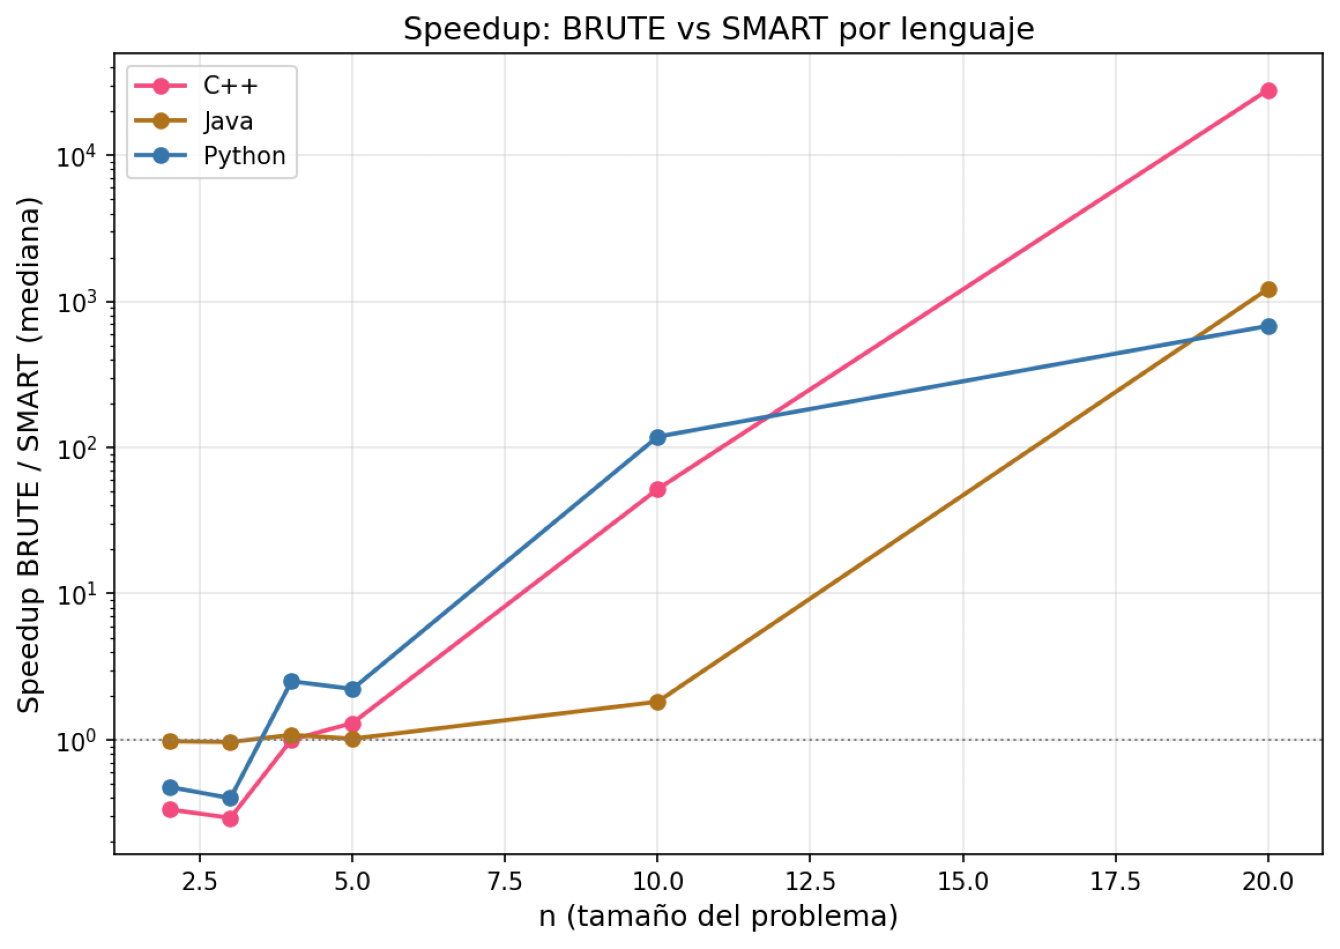
\includegraphics[width=\linewidth]{figuras/brute_vs_smart.pdf}
\end{center}
\end{column}

\begin{column}{0.41\textwidth}

\textbf{Cifras destacadas:}

\smallskip
\begin{block}{SMART vs BRUTE}
\small Speedup $> \mathbf{60\,000\times}$\\
para $n{=}20$, $m{=}80$
\end{block}

\smallskip
\begin{block}{Entre lenguajes (SMART, $n{=}30$)}
\small
\begin{tabular}{lr}
\textbf{C++}    & $18$ ms  \\
\textbf{Java}   & $52$ ms  \\
\textbf{Python} & $1\,150$ ms \\
\end{tabular}\\[2pt]
C++ vs Java: $\approx 3\times$\\
C++ vs Python: $\approx 63\times$
\end{block}

\smallskip
{\footnotesize\textit{Nodos explorados identicos en los 3 lenguajes (37\,854 para $n{=}30$, $m{=}120$).}}

\end{column}
\end{columns}

\end{frame}
